\documentclass[a4paper]{article}
\usepackage{tikz}
\usetikzlibrary{petri,arrows}
\usepackage{amstext}

\begin{document}


%% TikZ style options %%
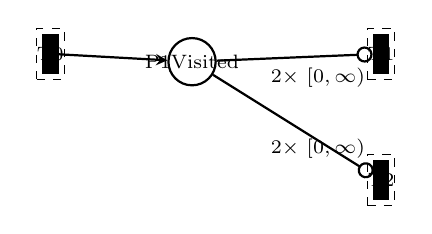
\begin{tikzpicture}[font=\scriptsize, xscale=1, yscale=1]
%% the figure can be scaled by changing xscale and yscale
%% positions of place/transition labels that are currently fixed to label=135 degrees
%% can be adjusted so that they do not cover arcs
%% similarly the curving of arcs can be done by adjusting bend left/right=XX
%% labels may be slightly skewed compared to the tapaal drawing due to rounding.
%% This can be adjusted by tuning the coordinates of the label
\tikzstyle{arc}=[->,>=stealth,thick]
\tikzstyle{transportArc}=[->,>=diamond,thick]
\tikzstyle{inhibArc}=[->,>=o,thick]
\tikzstyle{every place}=[minimum size=6mm,thick]
\tikzstyle{every transition} = [fill=black,minimum width=2mm,minimum height=5mm]
\tikzstyle{every token}=[fill=white,text=black]
\tikzstyle{sharedplace}=[place,minimum size=7.5mm,dashed,thin]
\tikzstyle{sharedtransition}=[transition, fill opacity=0, minimum width=3.5mm, minimum height=6.5mm,dashed]
\tikzstyle{urgenttransition}=[place,fill=white,minimum size=2.0mm,thin]\tikzstyle{uncontrollabletransition}=[transition,fill=white,draw=black,very thick]
%% TikZ-figure elements %%
\node[place] at (2.5,-2.2) (P1Visited) {};
%% label for place P1Visited
\draw (2.5,-2.2) node[align=left] {$\mathrm{P1Visited}$};
\node[transition] at (0.7,-2.1) (T0) {};
\node[sharedtransition] at (T0.center) { };
%% label for transition T0
\draw (0.7,-2.1) node  {$\mathrm{T0}$};
\node[transition] at (4.9,-2.1) (T1) {};
\node[sharedtransition] at (T1.center) { };
%% label for transition T1
\draw (4.9,-2.1) node  {$\mathrm{T1}$};
\node[transition] at (4.9,-3.7) (T2) {};
\node[sharedtransition] at (T2.center) { };
%% label for transition T2
\draw (4.9,-3.7) node  {$\mathrm{T2}$};
\draw[arc] (T0) to[bend right=0] (P1Visited) {};
\draw[inhibArc] (P1Visited) to[bend right=0] (T1) {};
%% Label for arc between P1Visited and T1
\draw (4.1,-2.4) node {$2\times$\ $\mathrm{[0,\infty)}$};
\draw[inhibArc] (P1Visited) to[bend right=0] (T2) {};
%% Label for arc between P1Visited and T2
\draw (4.1,-3.3) node {$2\times$\ $\mathrm{[0,\infty)}$};
\end{tikzpicture}
\end{document}
